%!TEX root = ../../main.tex

\chapter{Sequences}
\label{cha:sequences}

A sequence is a list of pictograms, where it is possible to mark a progress in the sequence of pictograms. This components is very common in the Sekvens app and the Ugeplan app.

\section{Progress}
\label{sec:progress}

The progress of the sequence is indicated by the size of pictograms in the sequence. The pictogram currently in progress is always in the middle of the view displaying the sequence as seen in \figref{fig:sequence_progress}. When displaying pictograms to a citizen it may not split (\secref{sub:citizen_view}). Upcomming pictograms should be a bit smaller than the one currently in progress. When progress has been made the pictograms that are done should be smaller and grayed as seen in \figref{fig:sequence_two} and \figref{fig:sequence_three}. For the ratio between the pictograms see \tabref{tab:sequence_ratio}.

\begin{figure}[!htbp]
    \centering

    \begin{subfigure}[t]{0.27\textwidth}
    	\centering
        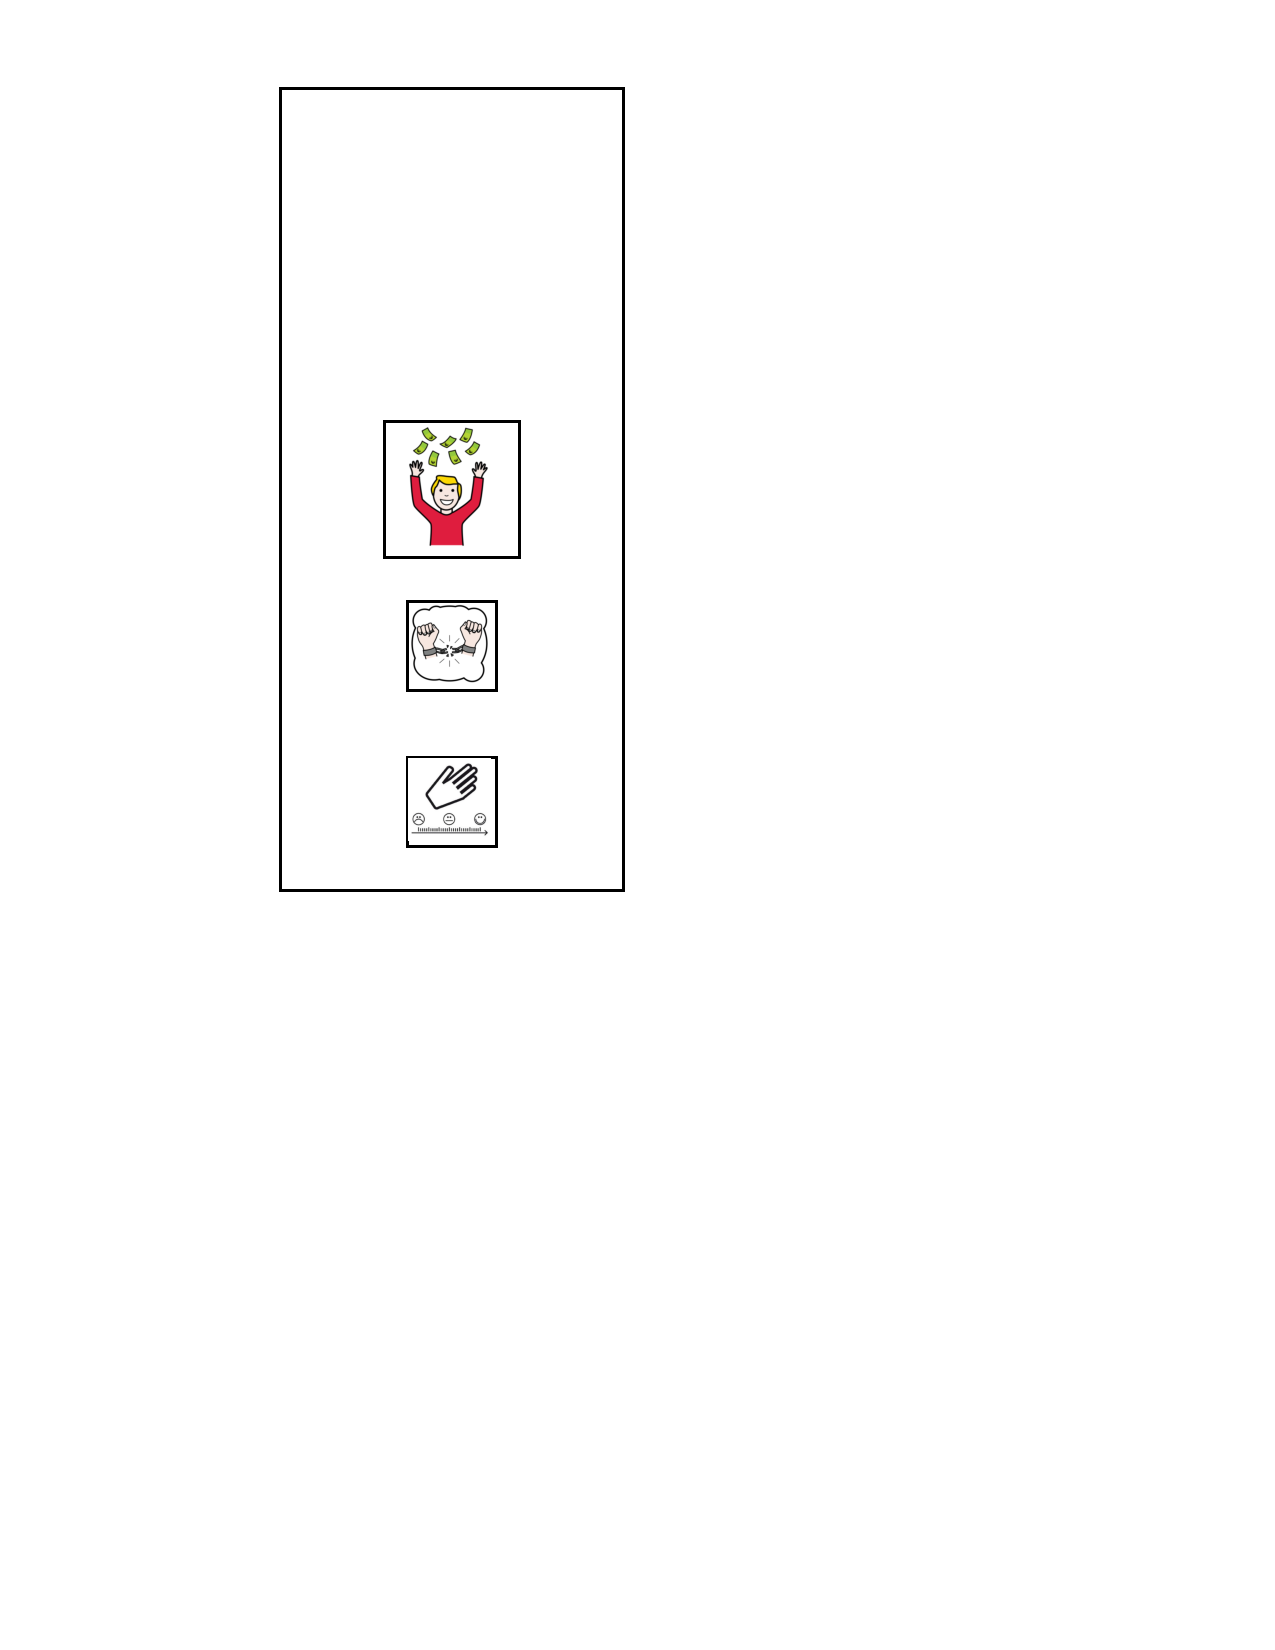
\includegraphics[scale=0.3]{sequence_one}
        \caption{Start of sequence}
        \label{fig:sequence_one}
    \end{subfigure}
    \hspace{2em} 
    \begin{subfigure}[t]{0.27\textwidth}
    	\centering
        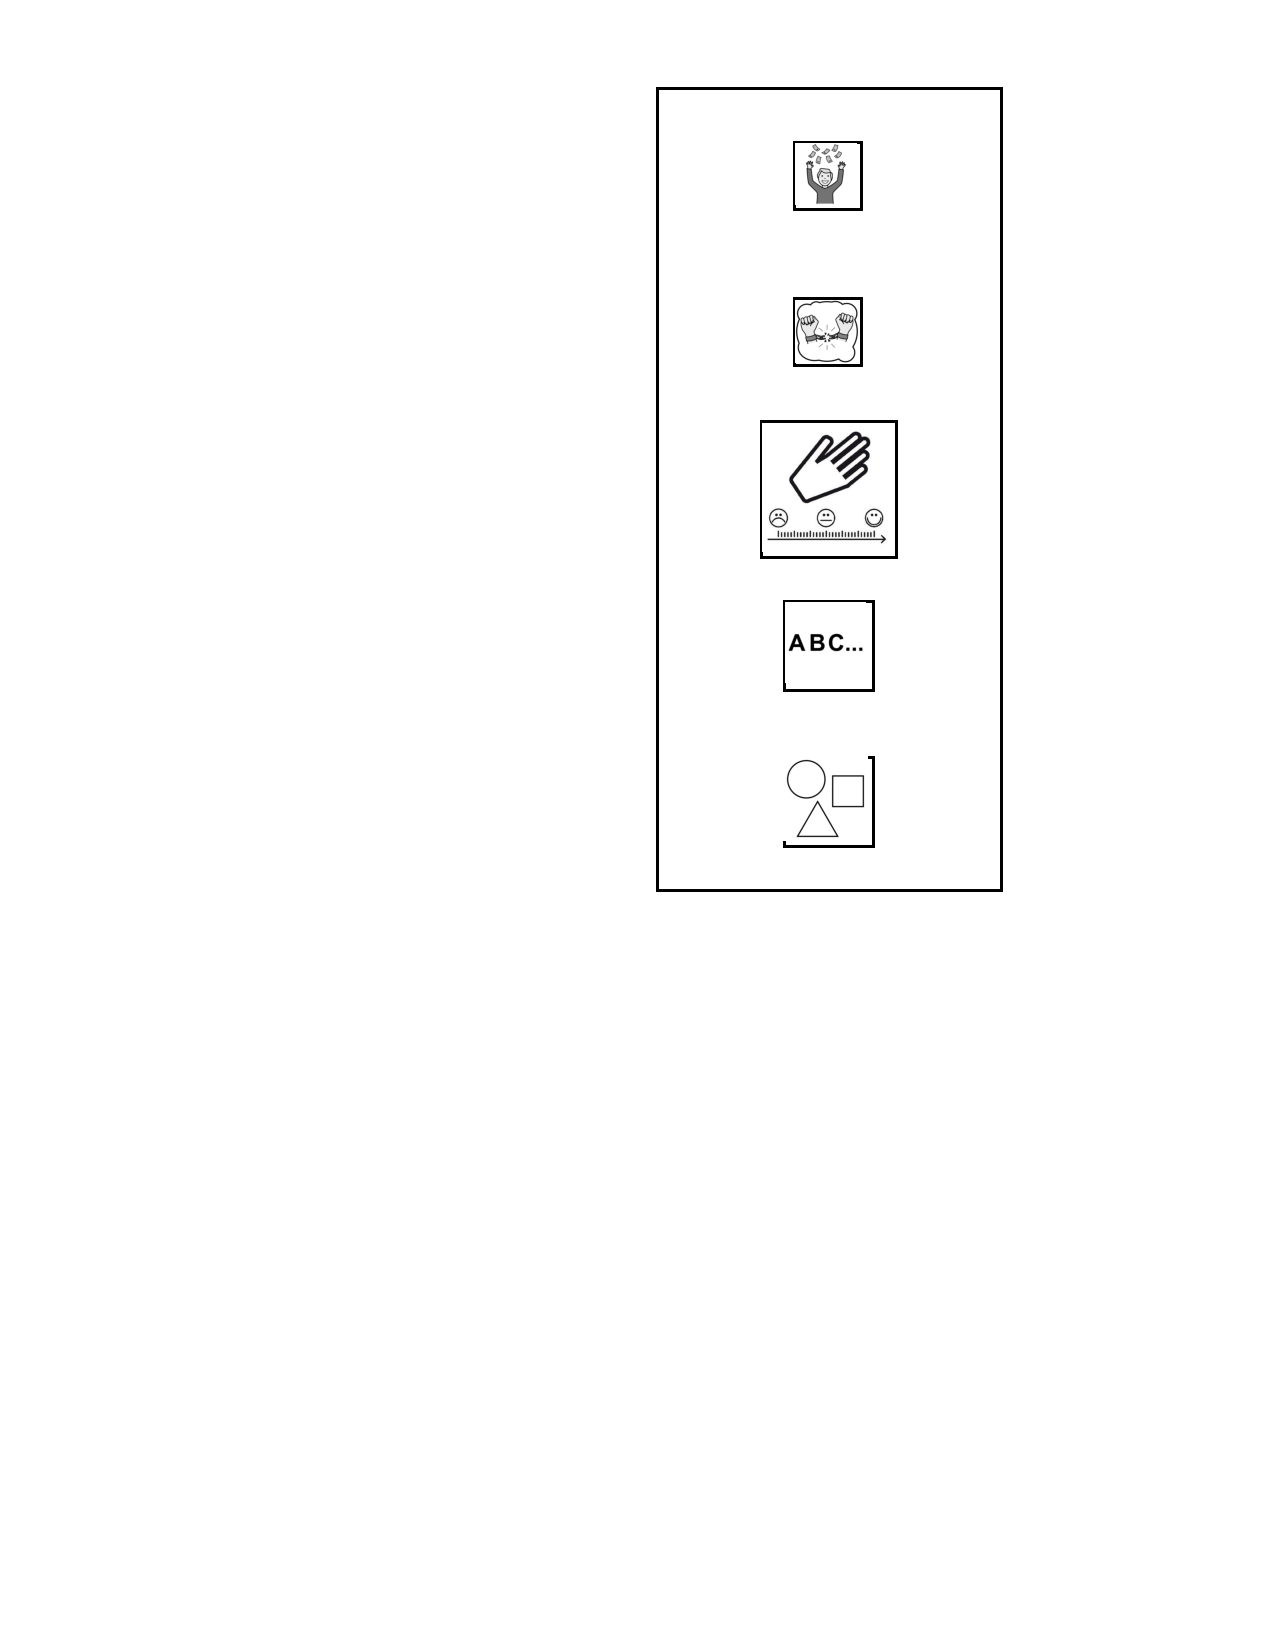
\includegraphics[scale=0.3]{sequence_two}
        \caption{Middle of sequence}
        \label{fig:sequence_two}
    \end{subfigure}
    \hspace{2em} 
    \begin{subfigure}[t]{0.27\textwidth}
    	\centering
        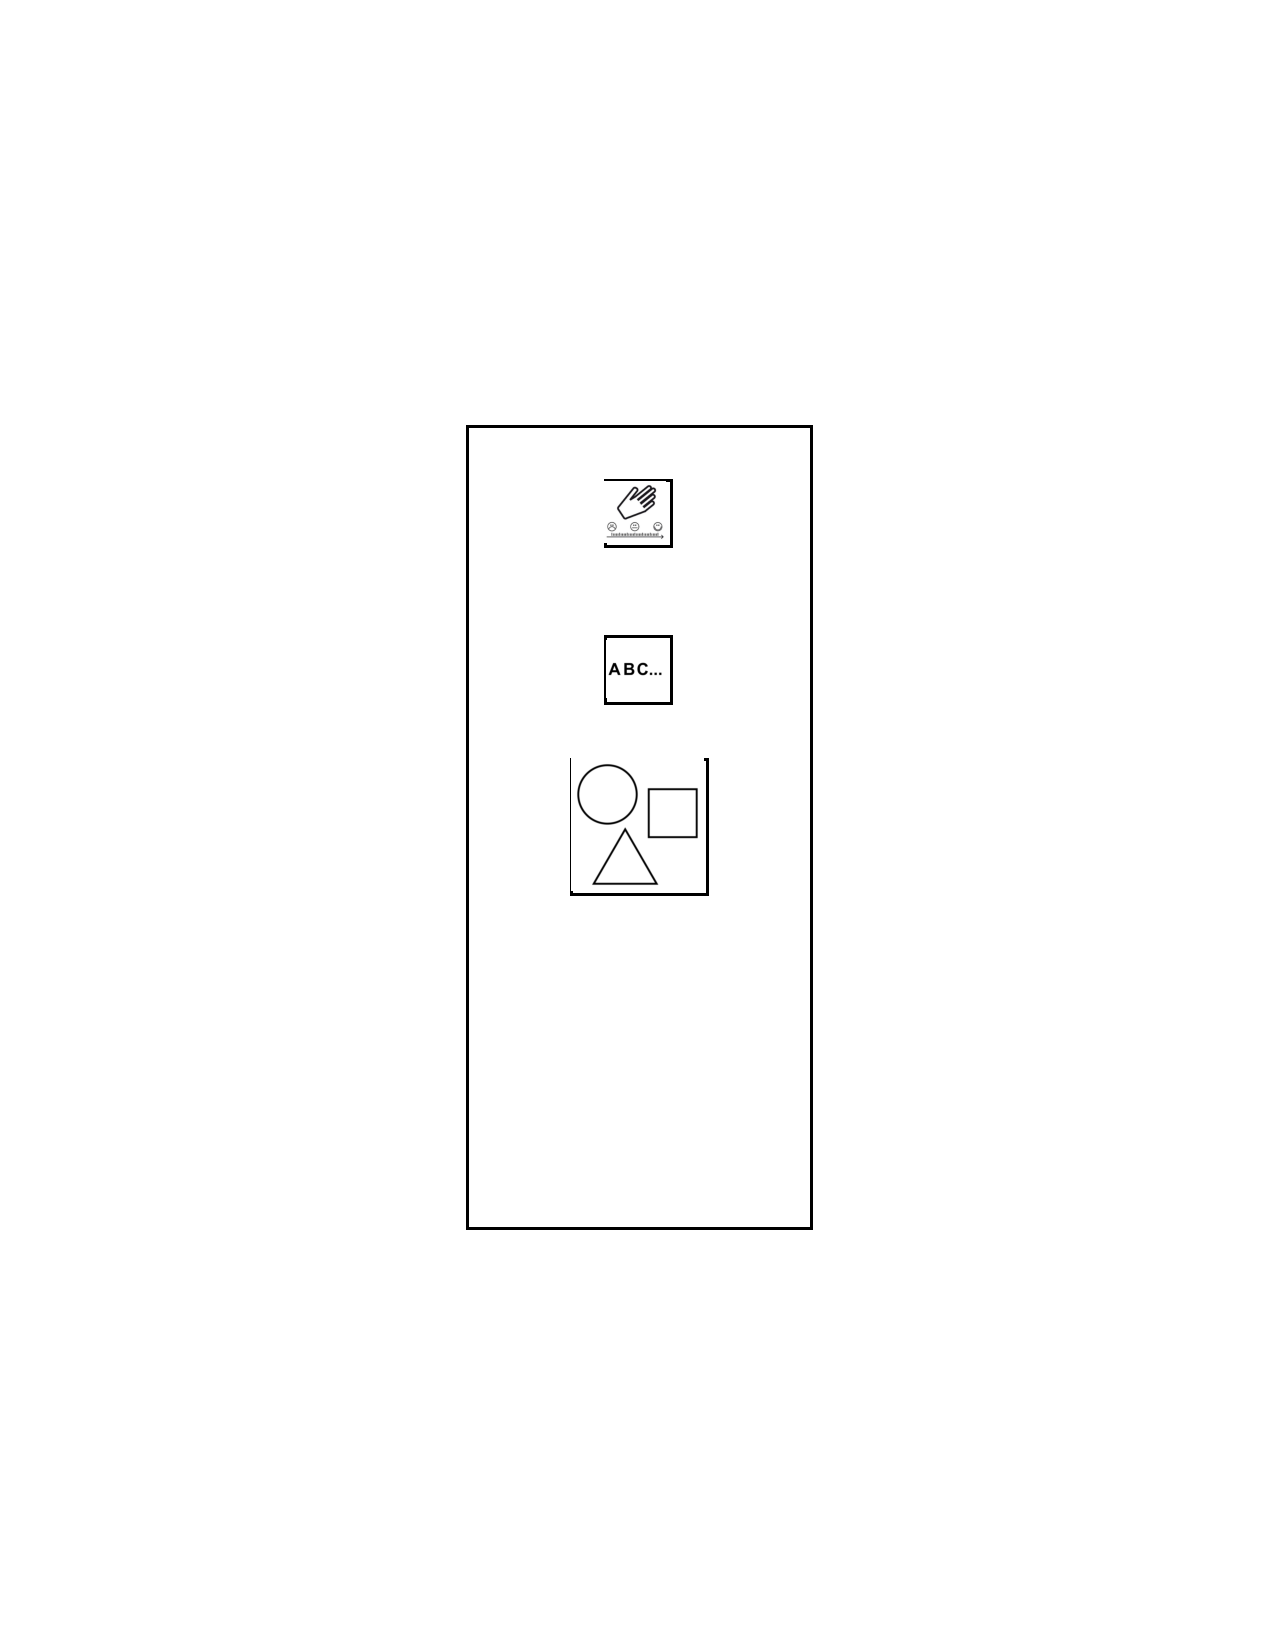
\includegraphics[scale=0.3]{sequence_three}
        \caption{End of sequence}
        \label{fig:sequence_three}
    \end{subfigure}
    
    \caption{Sequence progress}
    \label{fig:sequence_progress}
\end{figure}

\begin{table}[!htbp]
	\centering
	\begin{tabular}{|l|c|c|c|}
		\hline
		~ & Upcomming & In Progress & Done \\ \hline
		Ratio & 1 & 1.5 & 0.75 \\ \hline
	\end{tabular}
	\caption{Sequence picotgrams ratio}
    \label{tab:sequence_ratio}
\end{table}
